\documentclass[12pt, twocolumn]{report}
\usepackage{amsfonts}
\usepackage{amsmath}
\usepackage{amssymb}
\usepackage{caption}
\usepackage{subcaption}
\usepackage{setspace}
\usepackage{geometry}
\usepackage{hyperref}
\usepackage{graphicx}
\usepackage{listings}
\usepackage[lighttt]{lmodern}

\onehalfspacing
\geometry{margin=25mm}
\lstset{basicstyle=\ttfamily, keywordstyle=\bfseries}

\author{Liuchuyao Xu}
\title{General-purpose Computing on Graphics Processing Units for Real-time Analysis of Scanning Electron Microscope Images}

\begin{document}
\maketitle
\tableofcontents

\begin{abstract}
\end{abstract}

\chapter{Introduction}
\paragraph{}
The scanning electron microscope (SEM) is a type of microscope that produces images using signals generated from the interaction between electrons and the surface under observation. It has higher resolutions than traditional optical microscopes---an SEM can have a resolution lower than one nanometre, whereas that of an optical microscope is limited to a few hundred nanometres. This has benefited a variety of fields by allowing scientists to see micro-details of objects that were previously difficult or impossible to observe. For example, SEMs are an essential quality control tool for wafer manufacturing processes in the semiconductor industry \cite{SEM for semiconductor inspection}. A review SEM detects the defects on a die by comparing an image of it with a reference, and then stores the image for further use. The inspection would have been impossible without the aid of SEMs.

\paragraph{}
Fig. \ref{SEM basic construction} shows the basic construction of the SEM. The electron gun generates an electron beam, which is transformed into an electron probe after passing through the condenser lens and objective lens. It is scanned across the specimen under the effect of the scanning coil. As a result of the interaction between the incident electrons and the specimen, some electrons are emitted from the specimen. They are called secondary electrons and are collected by the detector, which generates signals based on their energy levels. The display unit converts the signals into images; one image is produced after each complete scan of the specimen.

\begin{figure}[htbp]
    \centering
    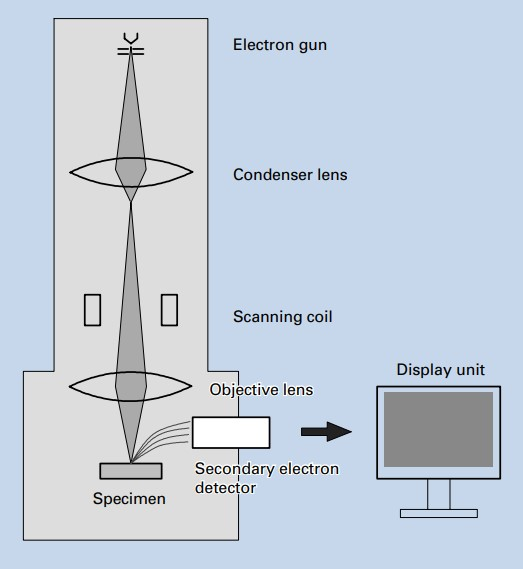
\includegraphics[width=0.49\textwidth]{Figures/SEM basic construction.jpg}
    \caption{Basic construction of the SEM \cite{SEM A to Z}.}
    \label{SEM basic construction}
\end{figure}

\paragraph{}
Many image analysis methods are used on SEM images. The fast Fourier transform is an especially important one since it can be used not only to study the structure of the specimen, but also to evaluate the focusing and astigmatism of the images [see section \ref{How the FFT can aid SEM operators}]; however, due to the complexity of the algorithm and a lack of fast hardware, real-time analysis had been either impossible or impractical in the past. In 1997, with an advanced central processing unit (CPU)---the Pentium Pro, it was only possible to achieve a refresh rate of 0.6 frames per second for 8-bit 1024 $\times$ 1024 input images \cite{SEM image sharpness measurement}. Although the enhancement of CPUs has enabled faster computations throughout the years, what really brings the speed to a different level is the development of graphics processing units (GPUs).

\paragraph{}
The GPU was originally designed to be a highly specialised hardware that excels in rendering complex, high-resolution, real-time 3D scenes for games; however, its special architecture has allowed it to outperform CPUs in many other areas and resulted in the birth of the idea of general-purpose computing on graphics processing units (GPGPU) \cite{GPU computing}, where GPUs are used to perform computations that are traditionally handled by CPUs.

\paragraph{}
A key characteristic of GPUs that differentiate them from CPUs is massive parallelism. Different pixels in a 3D scene require different processing to achieve visual effects such as lighting, blurring, and fogging. GPUs do this by breaking down the scene into fragments and manipulating each fragment independently. Modern GPUs have thousands of parallel processor cores each running tens of parallel threads to meet the requirement. For example, the NVIDIA GeForce GTX 1060 has 1280 cores and each of them is capable of running 16 threads; a similarly prices CPU---the Intel Core i7-7700HQ---has only 4 cores each running 8 threads. It is worth mentioning that the processing cores on a GPU are not as sophisticated as a full CPU and run at a lower clock frequency. The processor clock frequency of the GTX 1060 is 1708 MHz whereas the i7-7700 has a base processor frequency of 2800 MHz and a maximum of 3800 MHz. This means that GPGPU is more useful for applications that involve simple, repetitive, parallel tasks. A recent example is deep learning, where the same computation needs to be performed on a large network of nodes. Typical deep learning networks in 2015 consist of about one million nodes \cite{Deep learning}, which makes the computations impossible to be performed efficiently by CPUs.

\paragraph{}
This report studies the gain in computation speeds that can be obtained by using GPUs, and presents a real-time diagnostic tool made possible by that. The tool assists SEM operators by providing the histogram and FFT of the images in real-time. It was used to implement an automatic focusing and astigmatism correction algorithm for SEMs, and the performance is discussed.

\chapter{The gain in computation speeds from the use of GPUs}
\section{GPU computing}
\paragraph{}
GPUs are super parallel work distributors; they describe an image using a set of graphics primitives and allocate resources to manipulate each of them independently. Fig. \ref{GPU graphics primitives} shows the primitives used by modern GPUs. Different types of primitives are created and processed in different stages of the graphics pipeline, as described below:
\begin{itemize}
    \item Vertex fetching. The GPU fetches a list of vertices that represent the image as a 3D triangle mesh, as illustrated in Fig. \ref{GPU graphics triangle mesh}. Triangles are the fundamental hardware-supported primitive in modern GPUs; their advantage is that any of them can be defined by three vertices, which simplifies maths. Vertices are generated outside the GPU, together with information on lighting, texture, and transforms that need to be applied.
    \item Vertex shading. Mathematical operations are performed on the vertex data to add desired effects.
    \item Rasterisation. Each triangle is mapped to a block of pixels on the screen, called a ``fragment''.
    \item Fragment shading. The fragments are shaded on a per-pixel basis to determine their final colour.
    \item Raster operations. A final image is constructed by assembling the fragments and put into the frame buffer.
\end{itemize}
The processing units of the GPU support the data parallelism by adopting a single-program multiple-data (SPMD) programming model, where the same shading and rasterisation programs are used to to process different data. The programs can read data from shared global memory and write back to it. The GPU also makes use of task parallelism by dividing the pipe in \textit{space}, not time. Some pixels of a triangle could be running fragment-shading programs while others are already being written to the frame buffer; simultaneously, the GPU could be fetching the vertices of another triangle.

\begin{figure}[htbp]
    \centering
    \begin{subfigure}{0.45\textwidth}
        \centering
        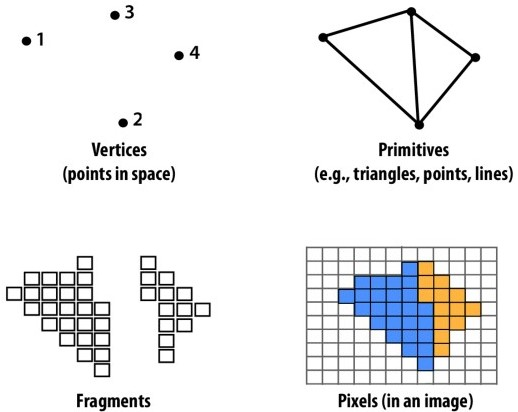
\includegraphics[width=1\textwidth]{Figures/GPU graphics primitives.jpg}
        \caption{Graphics primitives.}
        \label{GPU graphics primitives}
    \end{subfigure}
    \begin{subfigure}{0.45\textwidth}
        \centering
        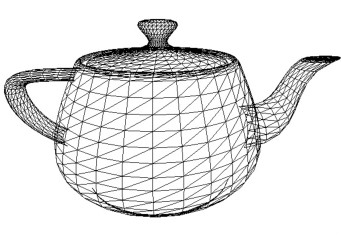
\includegraphics[width=1\textwidth]{Figures/GPU graphics triangle mesh.jpg}
        \caption{An image can be represented as a 3D triangle mesh.}
        \label{GPU graphics triangle mesh}
    \end{subfigure}
    \caption{The GPU describes an image as a set of primitives \cite{GPU architecture lecture}.}
    \label{GPU graphics}
\end{figure}

\paragraph{}
The parallelism can also provide a performance improvement for non-graphics tasks. Take the addition of two vectors of size $N$ as an example:
\begin{equation*}
    \boldsymbol{v_3} = \boldsymbol{v_1} + \boldsymbol{v_2}
\end{equation*}
A single-threaded CPU divides the task in time and does:
\begin{align*}
    & \text{Thread 1: }
\begin{cases}
    & \text{Time 1: } \boldsymbol{v_3}[0] = \boldsymbol{v_1}[0] + \boldsymbol{v_2}[0] \\
    & \vdots \\
    & \text{Time N: } \boldsymbol{v_3}[N] = \boldsymbol{v_1}[N] + \boldsymbol{v_2}[N] \\
\end{cases}
\end{align*}
This results in a time complexity of $O(N)$. The GPU can in theory achieve a time complexity of $O(1)$ by dividing the task among threads, and doing:
\begin{align*}
    & \text{Time 1: }
\begin{cases}
    & \text{Thread 1: } \boldsymbol{v_3}[0] = \boldsymbol{v_1}[0] + \boldsymbol{v_2}[0] \\
    & \vdots \\
    & \text{Thread n: } \boldsymbol{v_3}[N] = \boldsymbol{v_1}[N] + \boldsymbol{v_2}[N] \\
\end{cases}
\end{align*}
The vector addition is an SPMD task---each thread takes one element from each of the vectors and performs addition on them, but different threads handle different data. When $N$ is small, the overhead in allocating the threads means that the speed improvement is negligible; as $N$ grows larger, the reduction in time complexity quickly compensates for the overhead and makes the GPU much faster than the CPU; however, the GPU will run out of resources when $N$ is too big, and this sets a cap to its performance.

\paragraph{}
The vertex and fragment shading programs used to be fixed and graphics-specific, and the progression in making them customisable is a key that pushed the advancement of GPGPU \cite{GPU computing}. Prior to 2007, to use GPUs for general-purpose computing, the user must write programs using the language of the graphics application programming interface (API) since it was the only interface to GPU hardware:
\begin{itemize}
    \item The user specifies a list of ``vertices'' that cover a region on the screen.
    \item The user sets parameters of the graphics pipeline, e.g. ``lighting'' and ``texture''.
    \item The user provides ``shading'' programs for the vertices and fragments.
    \item The GPU produces an output ``image'' and stores it in global memory.
\end{itemize}
This was a major problem in GPGPU because many tasks have nothing to do with graphics and are difficult to translate into the graphics language. The introduction of CUDA changed the situation by providing a more natural, direct, non-graphics interface. The new programming model can be summarised as below:
\begin{itemize}
    \item The user defines the computation as a structured grid of threads.
    \item The GPU executes each thread and puts the result in global memory.
\end{itemize}
This eliminates the complexity in using the graphics API and allows the user to directly define threads that are run on the processing cores of the GPU.

\section{Experiment, results and discussions}
\paragraph{}
An experiment was conducted to determine the gain in computation speeds that can be obtained by using CUDA. A middle-range GPU---the NVIDIA GeForce GTX 1060---and a similarly priced CPU---the Intel Core i7-7700HQ---are used to perform addition of two random vectors of size $N$, which has a time complexity of $O(N)$ if done without parallelism.

\begin{figure*}[htbp]
    \centering
    \begin{subfigure}{0.7\textwidth}
        \centering
        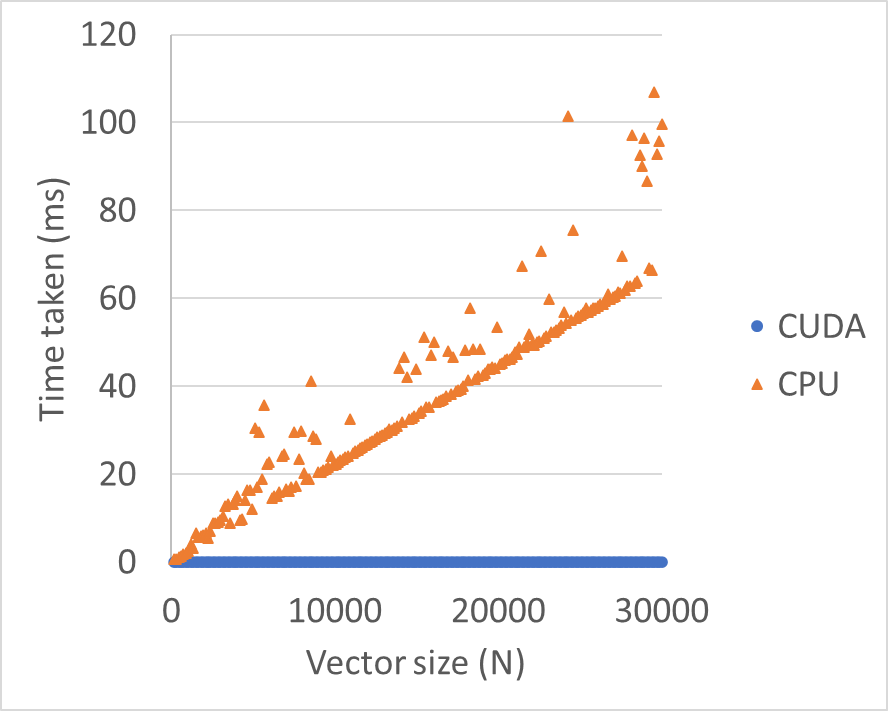
\includegraphics[width=1\textwidth]{Figures/Test vector addition GPU and CPU.png}
        \caption{Results of both the GPU and the CPU.}
        \label{Test vector addition GPU and CPU}
    \end{subfigure}
    \begin{subfigure}{0.45\textwidth}
        \centering
        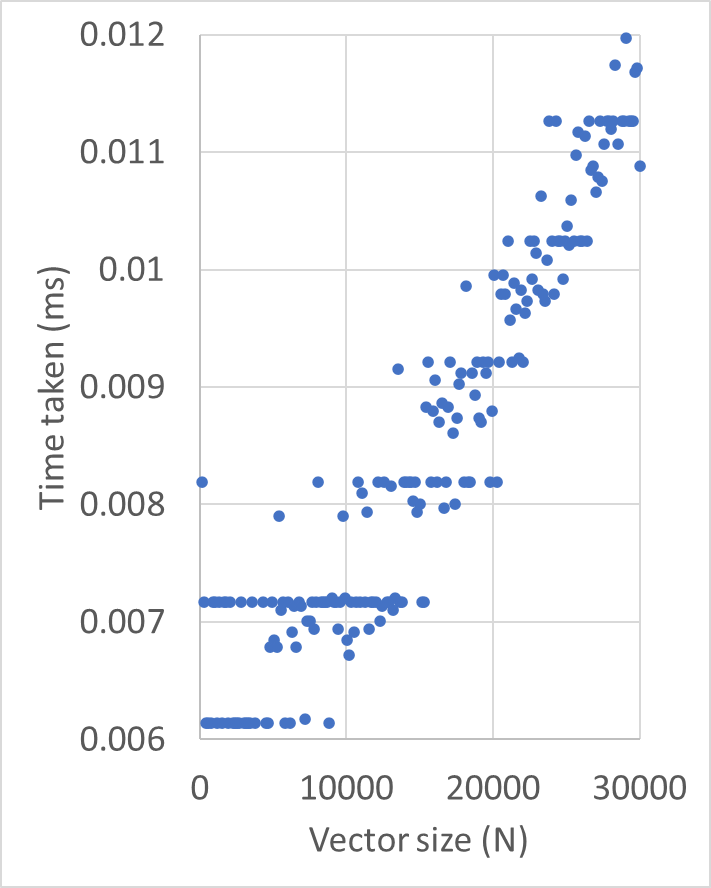
\includegraphics[width=1\textwidth]{Figures/Test vector addition GPU.png}
        \caption{Results of the GPU.}
        \label{Test vector addition GPU}
    \end{subfigure}
    \begin{subfigure}{0.45\textwidth}
        \centering
        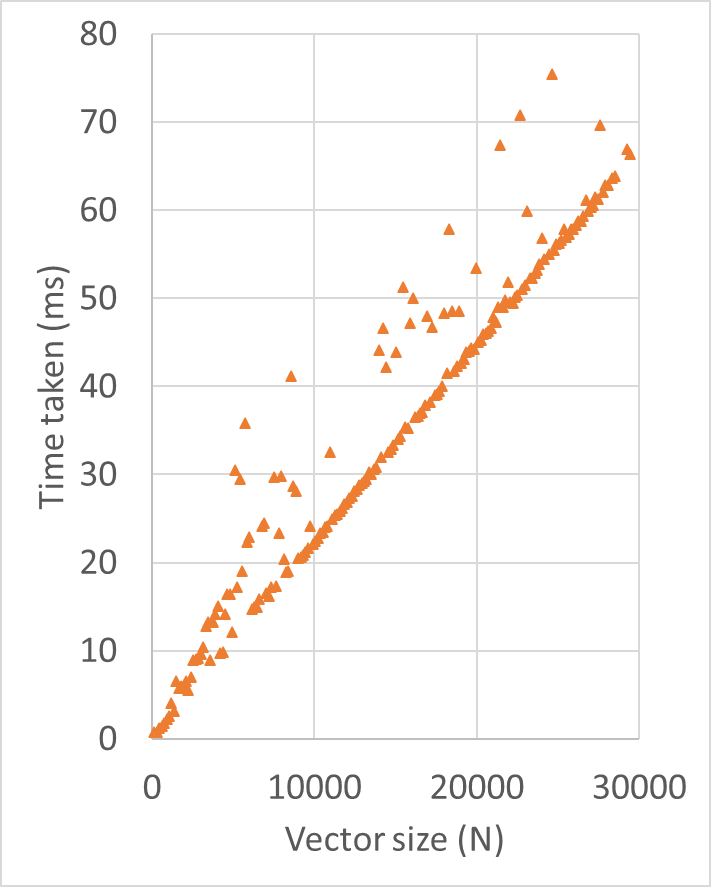
\includegraphics[width=1\textwidth]{Figures/Test vector addition CPU.png}
        \caption{Results of the CPU.}
        \label{Test vector addition CPU}
    \end{subfigure}
    \caption{Performance on vector addition of the GPU and the CPU}
    \label{Test vector addition}
\end{figure*}

\paragraph{}
Fig. \ref{Test vector addition} gives the results of the test. Measuring the gradient of the best-fit lines shows that the GPU is 12000 times faster, which agrees with the fact that the GPU is capable of running 20480 parallel threads while the CPU was only allowed to use one. It is possible to improve the performance of the CPU by making it use all of its 32 parallel threads, but it will still be hundreds of times slower. The maximum resolution of the GTX 1060 is 7680 $\times$ 4320 at 60 Hz, which means it can calculate two billion values within each second; if the Core i7 is used, that will take 200 minutes with one thread or 6 minutes with 32 threads.

\paragraph{}
Fig. \ref{Test vector addition GPU} shows that the computation time of the GPU does not scale linearly with the size of the vectors, but increases with steps. This confirms that the GPU can achieve time complexity of $O(1)$ within a limit, as described in the previous section.

\chapter{A real-time diagnostic tool for SEMs}
\section{Design of the software}
\paragraph{}
A diagnostic tool was developed based on fast computations provided by CUDA. The aim of the tool is to support interactive real-time diagnosis of SEM images that assists operators or automated procedures, and it has two main features:
\begin{itemize}
    \item Real-time histogram calculation.
    \item Real-time FFT calculation.
\end{itemize}

\paragraph{}
Considering that the tool may serve as the foundation stone for many further projects, the design of the software has a strong emphasis on readability and maintainability. This has affected the selection of programming language and the architecture of the software.

\paragraph{}
NVIDIA developed CUDA and provides an API for programmers to use it. The API is written in C and thus makes it a candidate programming language for developing the tool. Being a relatively low-level compiled language makes C extremely fast and useful for speed-critical applications. However, it also means that it has a complex syntax, which could significantly slow down development if the user does not have enough experience with it. Taking into account the time scale of the project and to make development easier for people who will continue the work, Python was used instead of C. It has a much simpler syntax and is widely supported; with careful design, it has proved to be able to produce useful results despite its slower speed.

\paragraph{}
% The software is highly modularised for maximising readability and maintainability. This also makes it easier to translate the program into C++ later if faster speed is needed since C++ is mostly used in an object-oriented manner. The software is divided into six main classes as shown in Fig. \ref{Software class diagram}:
To maximise quality, the software is highly modularised containing the following main classes:
\begin{itemize}
    \item \textit{SEM\_API}. This is a Python wrapper for the native SEM API written by Luyang Han, which allows the user to directly control the SEM and grab images from it in Python.
    \item \textit{SemImage}. This class encapsulates variables and methods that are directly relevant to SEM images. For example, it provides a function for applying a Hann window on the image, and a function for calculating the FFT of the image.
    \item \textit{SemImageGrabber}. This class provides a function for grabbing images from the SEM and creating instances of \textit{SemImage} from them. When an SEM can be detected, images are obtained by reading the memory of the SEM; otherwise, they are taken from a local folder specified by the user.
    % \item \textit{SemTool}. This class handles the rendering of the graphical user interface (GUI). Fig. \ref{Software GUI} shows a screenshot of the control panel. The pushbuttons open a window for the corresponding plot and the radio buttons select algorithms to be performed on the image. The plots are shown on different windows and can be opened and closed individually. This improves framerate by allowing the user to close unneeded windows, and also makes it easier to add other plots later. There are two ways for updating the plots, and the first one is to re-render the whole window. This wastes time since some components are always the same and do not need to be re-rendered, such as the window title and the axes. Therefore, \textit{SemTool} uses the second method, where only the data to be plotted are updated. This directly modifies the relevant data in the memory of the GPU, thereby avoiding re-rendering the whole window. Tests have shown that if the first method is used, the time taken to update each frame when there is only one plot opened will be 90 ms instead of 60 ms.
    \item \textit{SemTool}. This class handles the rendering of the graphical user interface (GUI); it is the entry point of the software. The user uses the GUI to specify which algorithms to be performed on the SEM images and what diagnostic information to be displayed.
    \item \textit{SemCorrector}. This class implements an automatic focusing and astigmatism correction algorithm for SEMs; it uses the \textit{Masker} class to ensure fast computing [see chapter \ref{An automatic focusing and astigmatism correction algorithm for SEMs}].
\end{itemize}

\paragraph{}
Fig. \ref{Software class diagram} shows the class diagram of the software. Dividing the software into multiple classes has many benefits, including the following:
\begin{itemize}
    \item The encapsulation of data and methods makes it easier to keep track of them, which improves readability. For example, \textit{SemImage} can be used as below:
    \begin{lstlisting}
image = semImageGrabber()
image.applyHanning()
image.updateFft()
image.updateHistogram()
    \end{lstlisting}
    \item It splits a big task into smaller ones, and thus improves maintainability by allowing the implementation of different tasks to be modified without changing other tasks. For example, \textit{SemImageGrabber} is implemented using 20 lines of code and used at four different places within \textit{SemCorrector}, by one line of code:
    \begin{lstlisting}
image = semImageGrabber()
    \end{lstlisting}
    Without \textit{SemImageGrabber}, \textit{SemCorrector} will require 76 more lines of code which all have to be changed whenever the programmer wants to implement a new method for grabbing images.
    \item Classes can be created by inheriting from other classes. This improves reusability by allowing subclasses to hold all the data and perform all the actions of their superclasses, and thus speeds up further developments.
\end{itemize}

\begin{figure}[htbp]
    \centering
    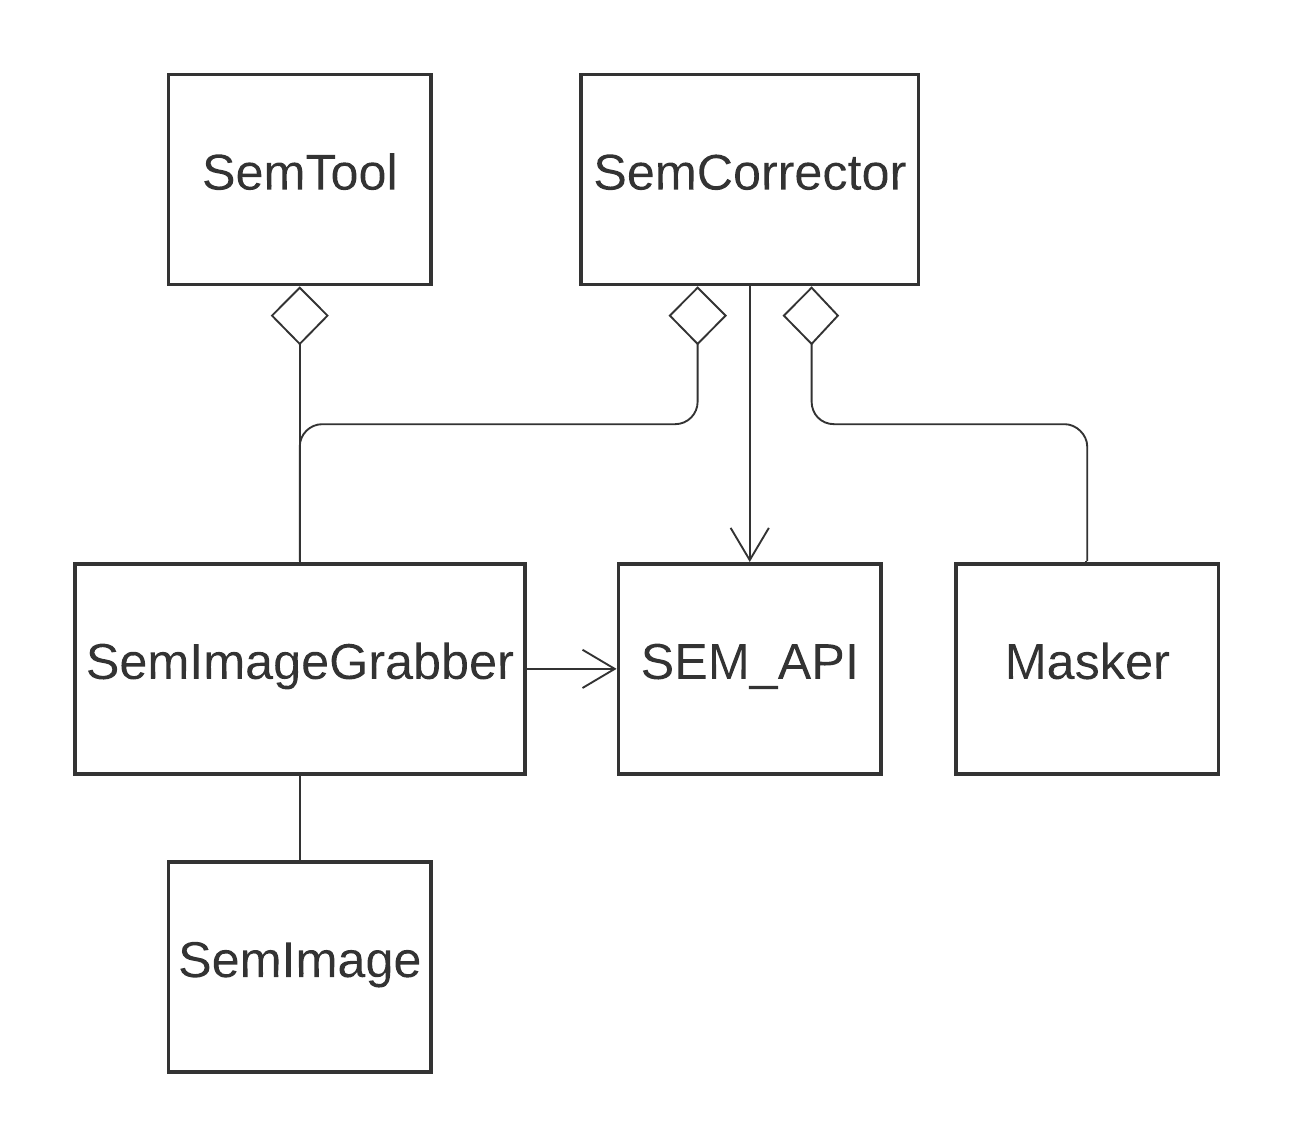
\includegraphics[width=0.45\textwidth]{Figures/Software class diagram.png}
    \caption{Class diagram of the software in unified modelling language (UML).}
    \label{Software class diagram}
\end{figure}

% \begin{figure}[htbp]
%     \centering
%     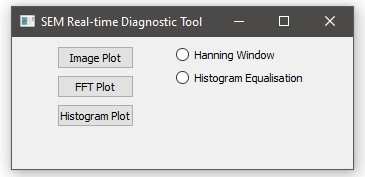
\includegraphics[width=0.45\textwidth]{Figures/Software screenshot.jpg}
%     \caption{Screenshot of the GUI.}
%     \label{Software GUI}
% \end{figure}

\section{Real-time histogram calculation}
\subsection{Theory of the histogram}
\paragraph{}
Histograms use bars to represent the shades of tones (level) that make up an image. The grey level (brightness level) histogram is the most relevant histogram to SEM images, since SEMs translate the energy of the secondary electrons directly into a grey level. The height of the bars in a grey level histogram can be calculated by
\begin{equation}
    n_l = \frac{1}{P} \sum_{p} I(l_p=l),
\end{equation}
where $n_l$ is the normalised number of pixels of grey level $l$, $P$ is the total number of pixels in the image and $l_p$ is the grey level of the $p_{th}$ pixel. 

\paragraph{}
Fig. \ref{Histogram equalisation inital image} shows an 8-bit grey-scale image, i.e. its depth of digitisation is 8-bit and it has 256 grey levels. Fig. \ref{Histogram equalisation inital image histogram} shows the histogram of the image and its integral. As can be seen in the histogram, most pixels are concentrated in the middle of the greyscale. This is reflected by the fact that the image is missing its highlights and shadows.

\begin{figure}[htbp]
    \centering
    \begin{subfigure}{0.4\textwidth}
        \centering
        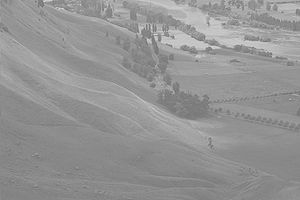
\includegraphics[width=1\textwidth]{Figures/Histogram equalisation inital image.jpg}
        \caption{Original image.}
        \label{Histogram equalisation inital image}
    \end{subfigure}
    \begin{subfigure}{0.4\textwidth}
        \centering
        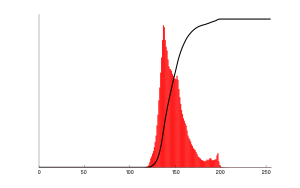
\includegraphics[width=1\textwidth]{Figures/Histogram equalisation inital image histogram.png}
        \caption{Histogram of the original image.}
        \label{Histogram equalisation inital image histogram}
    \end{subfigure}
    \begin{subfigure}{0.4\textwidth}
        \centering
        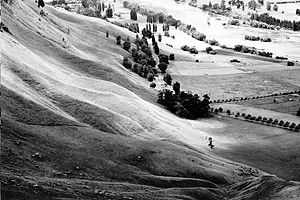
\includegraphics[width=1\textwidth]{Figures/Histogram equalisation final image.jpg}
        \caption{Histogram-equalised image.}
        \label{Histogram equalisation final image}
    \end{subfigure}
    \begin{subfigure}{0.4\textwidth}
        \centering
        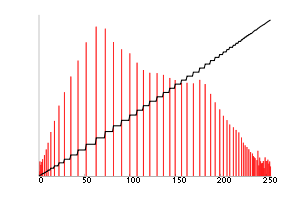
\includegraphics[width=1\textwidth]{Figures/Histogram equalisation final image histogram.png}
        \caption{Histogram of the histogram-equalised image.}
        \label{Histogram equalisation final image histogram}
    \end{subfigure}
    \caption{Histogram and histogram equalisation.}
    \label{Histogram and histogram equalisation}
\end{figure}

\subsection{How the histogram can aid SEM operators}
\paragraph{}
The contrast of an SEM image can be improved using histogram equalisation, which is a method for adjusting the distribution of pixel intensities of an image. Effectively, it is achieved by spreading out more frequent intensity values. To perform histogram equalisation, firstly obtain the integral of the histogram using
\[s_l = \sum_{i=1}^{l} n_i,\]
where $s_l$ is the value of the integral at grey level $l$. The integral spans from 0 to 1 as the histogram is normalised. Scale the integral by the maximum grey level and perform rounding to create the transform function
\begin{equation}
    f_l = \lfloor s_lL \rfloor,
    \label{Histogram equalisation transform function}
\end{equation}
If a pixel in the original image has a grey level $l$, it will have a grey level $f_l$ in the transformed image. For example, if all pixels in the original image are concentrated between grey level 100 to 200, the pixels of level 100 will become 0 in the new image while the pixels of level 200 will become 255 (assuming an 8-bit image).

\paragraph{}
The result is more noticeable when the image has low contrast, such as the one shown in Fig. \ref{Histogram equalisation inital image}. The histogram-equalised version of it is given in Fig. \ref{Histogram equalisation final image} and the new histogram in Fig. \ref{Histogram equalisation final image histogram}. More details are now visible as the contrast has been enhanced.

\subsection{A demonstration of GPU programming}
\paragraph{}
The most time-consuming part of histogram equalisation is to map all pixels in the original image to their new values using the transform function \eqref{Histogram equalisation transform function}. This can be implemented using CPU code in one line:
\begin{lstlisting}
newImage = 
  map(lambda x: f[x], image)
\end{lstlisting}
\lstinline{f} is an array that serves as the transformation function, if the original pixel value is x, the new value should be \lstinline{f[x]}. The \lstinline{lambda} operator is a way to create small anonymous functions, which are throw-away and are only needed where they are created. It improves conciseness and readability by reducing code bloat. \lstinline{lambda x: f[x]} creates an anonymous function that returns \lstinline{f[x]} when given \lstinline{x}, and \lstinline{map()} uses this function to transform all pixels in \lstinline{image}. This gives a time complexity of $O(N^2)$ which is not optimal. A smaller time complexity can be achieved using the GPU code:
\begin{lstlisting}
map = cupy.ElementwiseKernel(
  'T x, raw T f', 'T xNew',
  'xNew = f[x]',
  'map'
)
newImage = map(image, f)
\end{lstlisting}
\lstinline{cupy.ElementwiseKernel()} defines a kernel that the GPU uses to process the input data in parallel. Tests have shown that the use of GPU can increase the speed by 2 times, as summarised in Table \ref{Software performance test}. In theory, the factor of speed improvement should be similar as that for calculating the histogram, since it also requires iterating through all pixels in the image. However, the code implementations introduce overheads which limit the improvement in speed.

\section{Real-time FFT calculation}
\subsection{Theory of the FFT}
\paragraph{}
The Fourier transform (FT) decomposes a function into its constituent frequencies, as illustrated in Fig. \ref{FT demonstration}. The composite wave can be represented by the superposition of a 1 Hz sine wave and a 10 Hz sine wave, and its FT therefore has two components. A function that changes more abruptly will have stronger high-frequency components than a smoother one.

\begin{figure}[htbp]
    \centering
    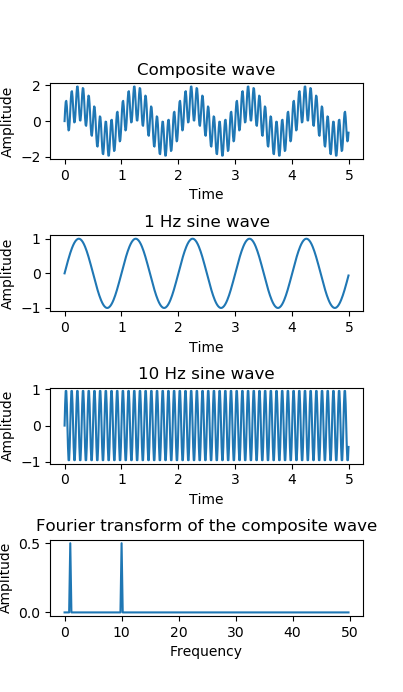
\includegraphics[width=0.45\textwidth]{Figures/FT demonstration.png}
    \caption{Fourier transform}
    \label{FT demonstration}
\end{figure}

\paragraph{}
In image processing, the discrete Fourier transform (DFT) is used instead of the FT, which takes a finite sequence of equally-spaced values as input and is thus better suited than the FT. It is defined by
\begin{equation}
    X_k = \sum_{n=0}^{N-1} x_n \cdot e^{-i2\pi kn/N}, \quad 0 \leq k \leq N-1,
    \label{FT DFT}
\end{equation}
where $x_0,x_1,...,x_{N-1}$ is the input sequence and $X_0,X_1,...,X_{N-1}$ is the output sequence. $X_k$ is effectively the result of the dot product between the vector $[x_0,x_1,...,x_{N-1}]$ and $[e^0,e^{-i2\pi k/N},...,,e^{-i2\pi k(N-1)/N}]$, and the latter is a finite sequence of frequency $2\pi k$. Therefore, the DFT computes the magnitude of the component of the input sequence that has frequency $2\pi k$, for $0 \leq k \leq N-1$.

\paragraph{}
A drawback of using \eqref{FT DFT} is that it has a time complexity of $O(N^2)$ ($N$ multiplications need to be computed for each of the $N$ components in the output sequence $X_0,X_1,...,X_{N-1}$). In image processing, where the inputs are 2D sequences, the time complexity quickly explodes and makes the equation practically impossible to use. A fast Fourier transform (FFT) is an algorithm that computes the DFT with smaller timer complexity. There are many feasible FFT algorithms and the most common one is the Cooley-Tukey algorithm \cite{FT FFT}. The algorithm is used where $N$ is, or can be chosen to be, a highly composite number. Suppose $N = r_1 \cdot r_2$, then the indices in \eqref{FT DFT} can be expressed as
\begin{align*}
    n = n_1r_2 + n_0, \quad & n_0 = 0, 1, ..., r_2 - 1, \\
    & n_1 = 0, 1, ..., r_1 - 1.
\end{align*}
Equation \eqref{FT DFT} can then be written as
\begin{align*}
    % X_k & = \sum_{n_0}\sum_{n_1} x_{n_0 + n_1} \cdot e^{-i2\pi k(n_1r_2 + n_0)/N} \\
    X_k & = \sum_{n_0}\sum_{n_1} x_{n_0 + n_1} \cdot e^{-i2\pi kn_1r_2/N} e^{-i2\pi kn_0/N} \\
    % & = \sum_{n_0}\sum_{n_1} x_{n_0 + n_1} \cdot e^{-i2\pi k_0(n_1r_2)/N} e^{-i2\pi k(n_0)/N} \\
    & = \sum_{n_0} e^{-i2\pi kn_0/N} \sum_{n_1} x_{n_0 + n_1} \cdot e^{-i2\pi kn_1r_2/N}.
\end{align*}
Now, only $r_1 + r_2$ operations need to be performed to compute $X_k$, and the whole algorithm requires $N(r_1 + r_2)$ operations. The procedure can be repeated to produce an $m$-step algorithm requiring $N(r_1 + r_2 + \cdots + r_m)$ operations, where $N = r_1 \cdot r_2 \cdots r_m$. Modern processors can perform the algorithm the most efficiently when $r_1 = r_2 = \cdots = r_m = 2$ because of their binary architecture, then the total number of operations is
\begin{align*}
    2N\log_2 N,
\end{align*}
which yields a time complexity of $O(N\log N)$. 

\paragraph{}
Fig. \ref{FT FFT on images} gives an example of FFT applied to a real image. The top row shows a set of images and the bottom row shows the corresponding transform (amplitudes only). Points near the origin represent lower-frequency components and are cut off when a high-pass filter is applied to the image.

\begin{figure}[htbp]
    \centering
    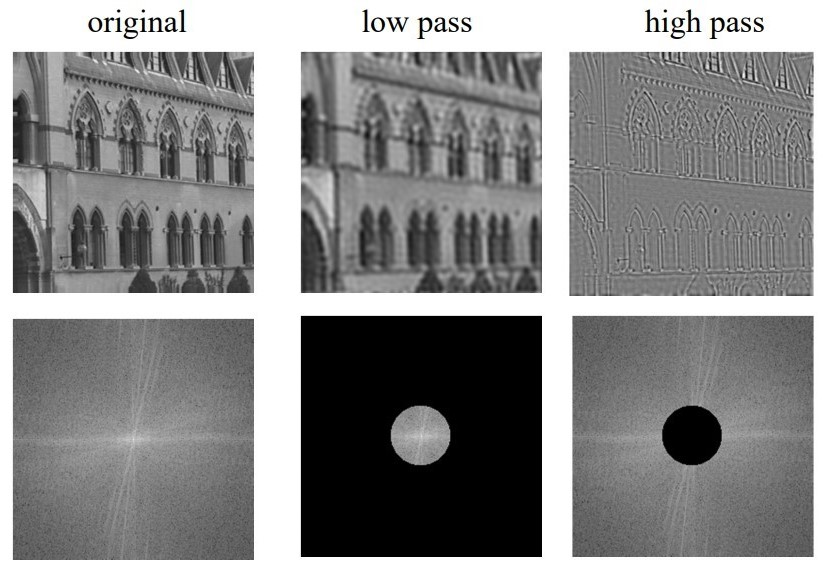
\includegraphics[width=0.45\textwidth]{Figures/FT FFT on images cropped.jpg}
    \caption{FFT and filtering on images \cite{FT lecture}.}
    \label{FT FFT on images}
\end{figure}

\paragraph{}
A problem in the use of the FFT for image analysis is the boundary effect. The abrupt discontinuity at the edges gives the FFT some strong high-frequency components. In practice, windows functions such as the Hann window and the Hamming window are often applied to the image before performing the FFT, which taper the edges off towards zero and thus reduce the boundary effect. Fig. \ref{FT window functions} shows how the Hann window and the Hamming window look like; they can be obtained by setting $a_0$ to $0.5$ and $25/46$, respectively, in the function
\begin{equation}
    w[n] = a_0 - (1-a_0)\cdot \cos{\frac{2\pi n}{N}}, \quad 0\leq n \leq N.
\end{equation}

\begin{figure}[htbp]
    \centering
    \begin{subfigure}{0.45\textwidth}
        \centering
        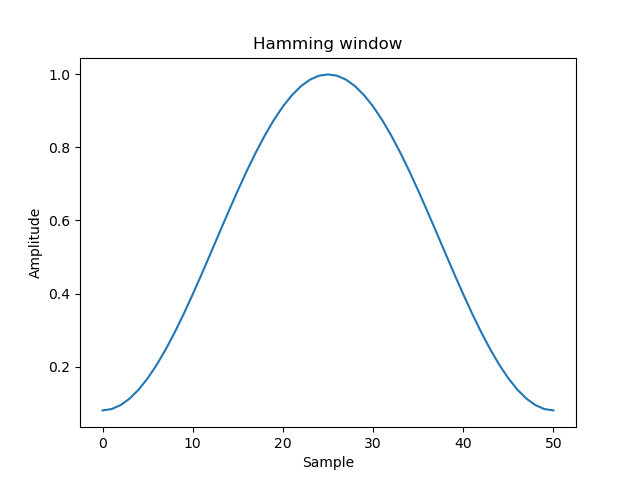
\includegraphics[width=1\textwidth]{Figures/FT window Hamming.png}
        \caption{Hamming window.}
    \end{subfigure}
    \begin{subfigure}{0.45\textwidth}
        \centering
        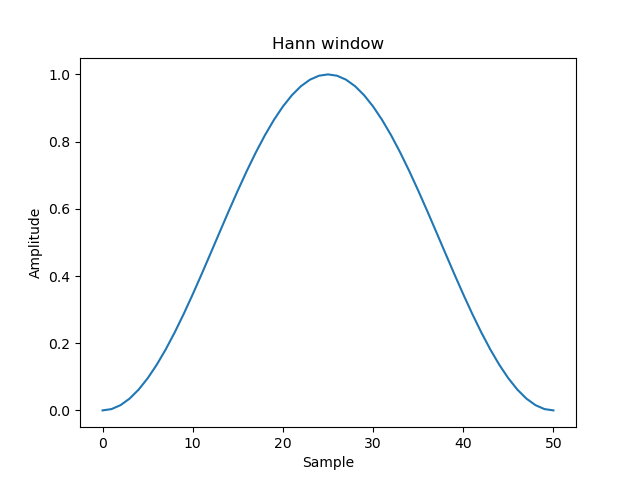
\includegraphics[width=1\textwidth]{Figures/FT window Hann.png}
        \caption{Hanning window.}
    \end{subfigure}
    \caption{Window functions.}
    \label{FT window functions}
\end{figure}

\subsection{How the FFT can aid SEM operators} \label{How the FFT can aid SEM operators}
\paragraph{}
The quality of an SEM image is affected by aberrations. While some exist because of the fundamental properties of the microscope and are difficult to get rid of, some can be eliminated by adjusting relevant settings. Two important ones are focus and stigmator control, which directly affect the resolution and astigmatism of the image, respectively. Fig. \ref{SEM sample images} illustrates the effect of wrong focus and stigmator settings.

\begin{figure}[htbp]
    \centering
    \begin{subfigure}{0.45\textwidth}
        \centering
        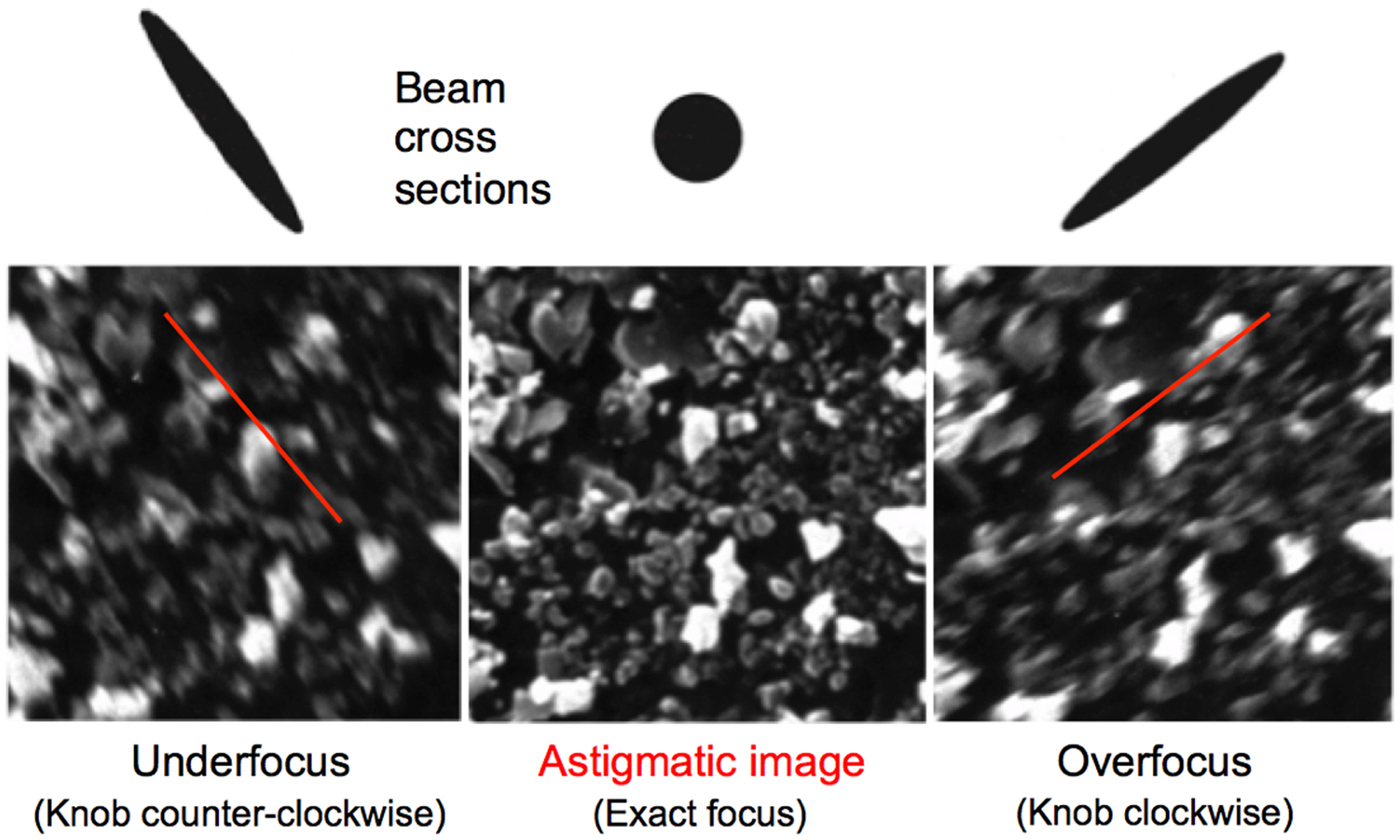
\includegraphics[width=1\textwidth]{Figures/SEM sample images astigmatism a.jpeg}
        \caption{Astigmatic images with different level of focusing.}
    \end{subfigure}
    \begin{subfigure}{0.45\textwidth}
        \centering
        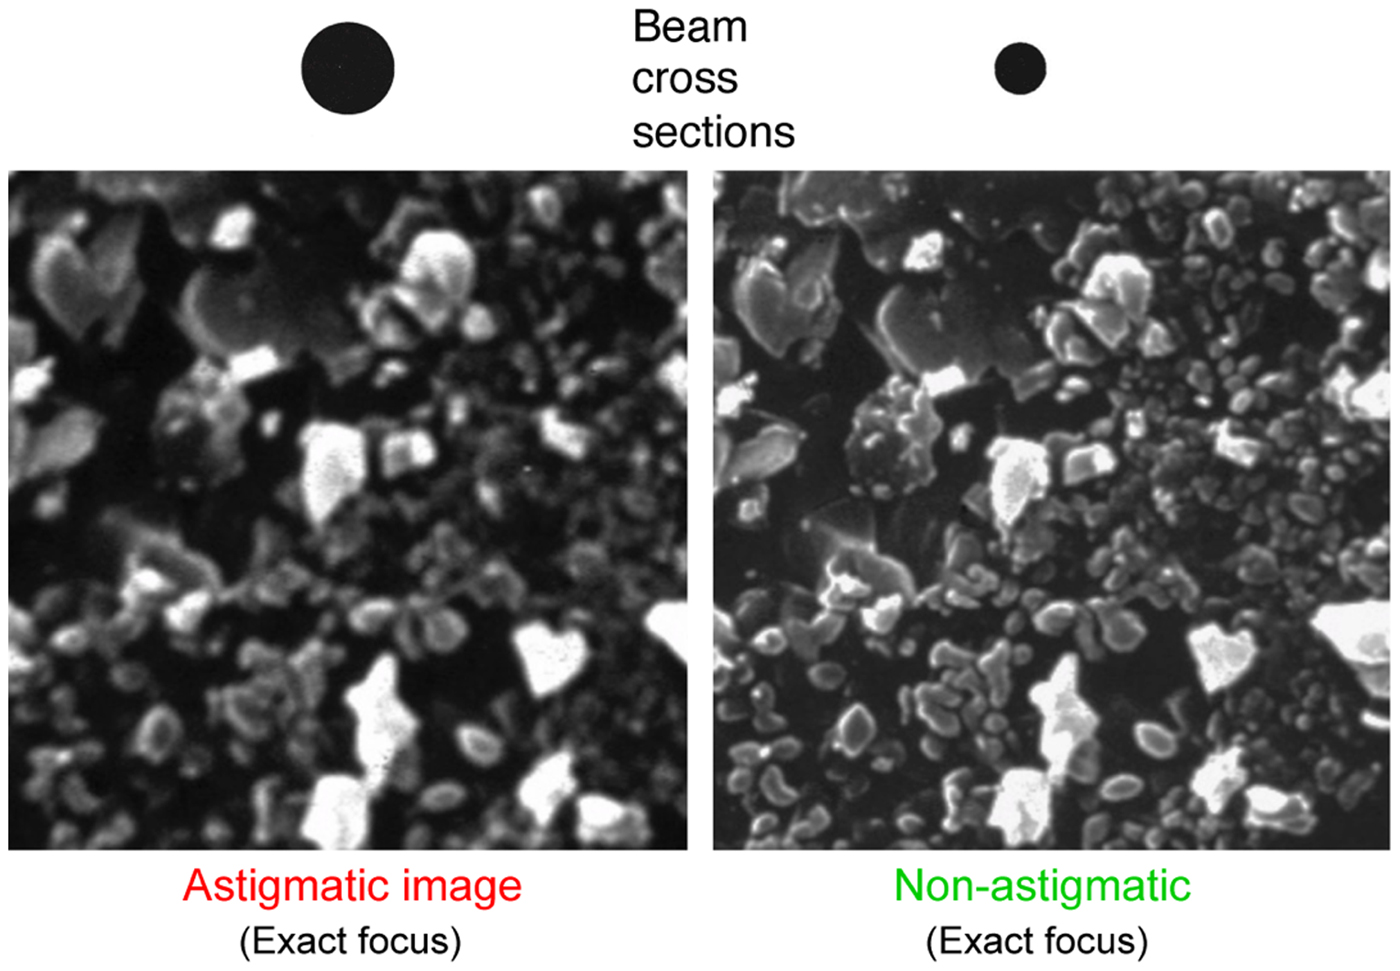
\includegraphics[width=1\textwidth]{Figures/SEM sample images astigmatism b.jpeg}
        \caption{Exact-focus images with different level of astigmatism.}
    \end{subfigure}
    \caption{Sample astigmatic SEM images \cite{SEM astigmatism correction}.}
    \label{SEM sample images}
\end{figure}

\paragraph{}
Focus determines the focal point of the electron probe. When the focal point is far from the surface of the specimen, the incident electrons interact with the specimen in a larger area. As a result, spots near each other produce signals of closer magnitude. This makes the image appear blurry.

\paragraph{}
Stigmators are used to compensate for astigmatism. Astigmatism arises due to imperfections in components of the SEM and describes uneven focus in the electron probe, as illustrated in Fig. \ref{SEM uneven focus}. When the electron probe is out of focus, astigmatism makes the incident electrons interact with the specimen in an elliptical area, and thus makes the image appear stretched. When the electron probe is in focus, astigmatism makes the image appear blurry.

\begin{figure}[htbp]
    \centering
    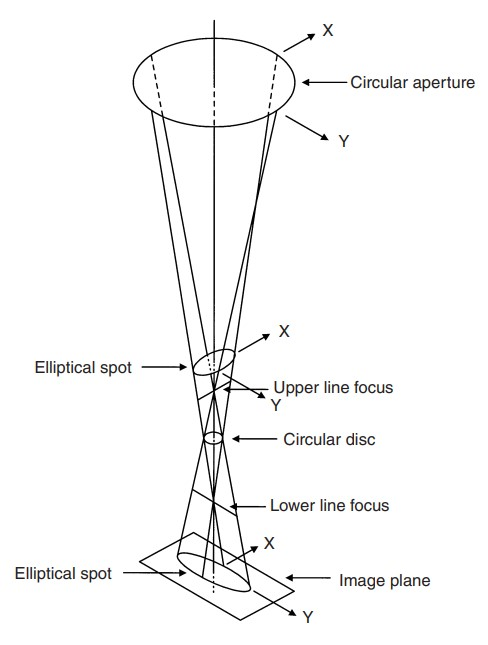
\includegraphics[width=0.45\textwidth]{Figures/SEM uneven focus.jpg}
    \caption{Uneven focus of the SEM.}
    \label{SEM uneven focus}
\end{figure}

\paragraph{}
Although experienced SEM operators can often tell the accuracy of focusing and level of astigmatism in a short time, it may not be as straightforward for new users. The complexity arises because any judgement of an image is based on what the operators see through their eyes, which is subjective. Sometimes, the surface being observed may have a complex structure and makes judgement even harder. Intensive training and practical experience are often required for an operator to become efficient in using the SEM.

\paragraph{}
The real-time FFT calculation aids the operators by providing an alternative way of evaluating the focusing and astigmatism of images using the FFT. Fig. \ref{SEM astigmatism} provides a set of sample images that illustrate how different degrees of defocus and astigmatism affect the FFT of an image. An in-focus image contains more details, and its FFT will thus have stronger high-frequency components. The FFT of an astigmatic image rotates by 90 degrees as the image goes from under-focus from over-focus; this is because the elliptical incidence area of the electron probe rotates by 90 degrees and makes the image appear stretched in the new direction (as shown in Fig. \ref{SEM sample images}).

\begin{figure*}
    \centering
    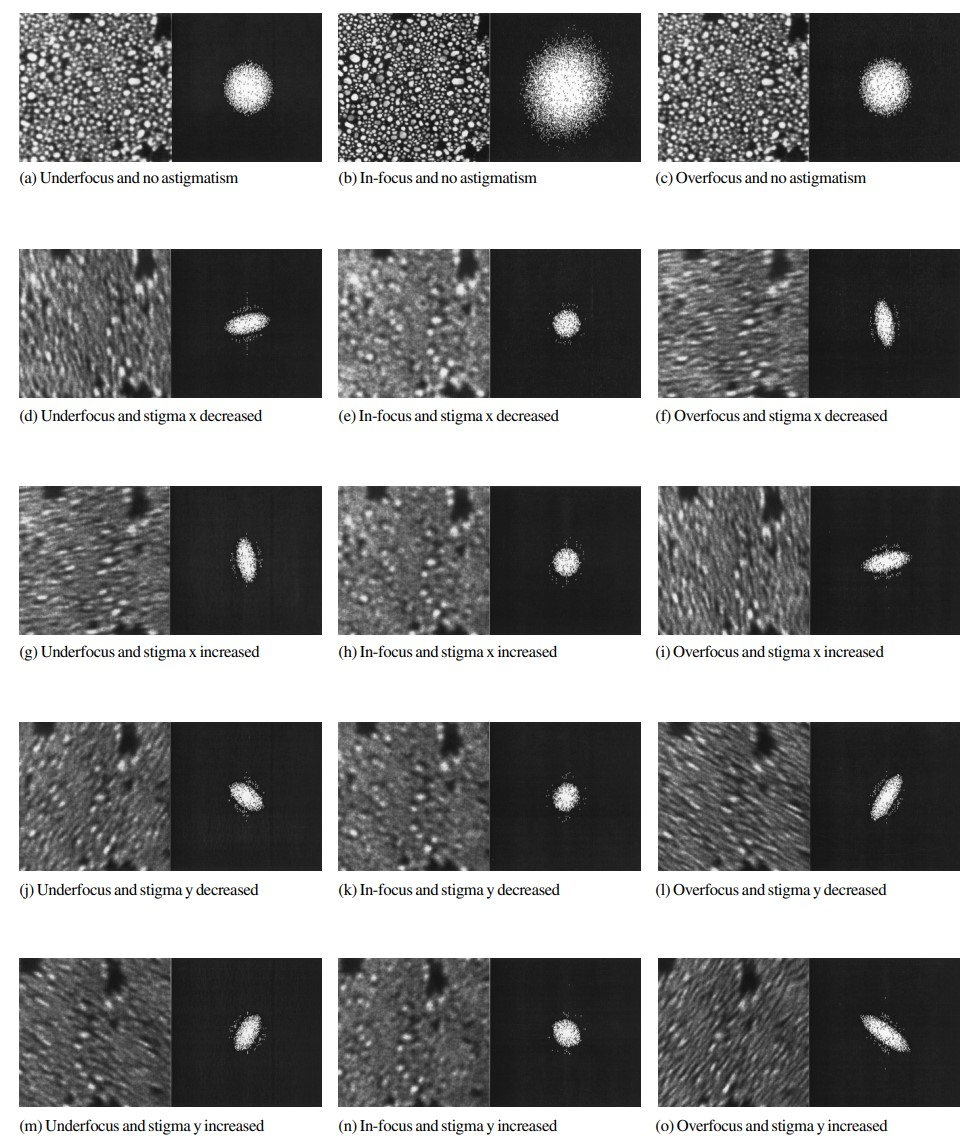
\includegraphics[width=1.05\textwidth]{Figures/SEM astigmatism and FFT.jpg}
    \caption{Images of gold-on-carbon sample and their fast Fourier transforms (FFTs) for different degrees of defocus and astigmatism \cite{SEM correction algorithm}.}
    \label{SEM astigmatism}
\end{figure*}

\paragraph{}
The importance of real-time calculation is that it saves SEM operators time by eliminating the need for downloading each image, and thus improves their productivity.

\section{Performance tests of the tool}
\paragraph{}
Experiments were conducted to test the performance of the tool with the NVIDIA GeForce GTX 1060 and the Intel Core i7. The following algorithms were performed on a set of 8-bit 1024 $\times$ 768 SEM images and the average results are shown in table \ref{Software performance test}. If all the algorithms need to be performed on each image, using the CPU will limit the framerate to about 9 fps. The use of GPU changes the number to 42 fps, which gives margin to other processes such as the rendering of the GUI.

\begin{table}[htbp]
    \caption{Results of performance tests of the diagnostic tool}
    \begin{center}
    \begin{tabular}{|c|c|c|}
    \hline
    \textbf{Algorithm} & \textbf{CPU} & \textbf{GPU} \\
    \hline
    Apply Hanning window & 16 ms & 9 ms \\
    \hline
    Calculating histogram & 30 ms & 2 ms \\
    \hline
    Histogram equalisation & 9 ms & 5 ms \\
    \hline
    Fast Fourier transform & 60 ms & 8 ms \\
    \hline
    \end{tabular}
    \label{Software performance test}
    \end{center}
\end{table}

\chapter{An automatic focusing and astigmatism correction algorithm for SEMs} \label{An automatic focusing and astigmatism correction algorithm for SEMs}
\section{Theory of the algorithm}
\paragraph{}
K.H. Ong, J.C.H. Phang, and J.T.L. Thong proposed an algorithm for automatically correcting the focusing and astigmatism of the SEM \cite{SEM correction algorithm}, which uses the properties of the FFT of SEM images described in section \ref{How the FFT can aid SEM operators}.

\paragraph{}
Firstly, convert the FFT of the image into a binray image by applying a threshold to the magnitudes, and then segment it into eight regions as shown in Fig. \ref{Correction algorithm FFT segmentation}. A pixel has value 1 if the magnitude is above the threshold and 0 otherwise. Let $I$ be a matrix representing the current image with focus set to $F$, obtain an under-focused image $I_{uf}$ and an over-focused image $I_{of}$ by setting the focus to $F-\Delta F=F_{uf}$ and $F+\Delta F=F_{of}$, respectively. Let $T$, $T_{uf}$ and $T_{of}$ be matrices representing the binary FFT of $I$, $I_{uf}$ and $I_{of}$, respectively.

\begin{figure}[htbp]
    \centering
    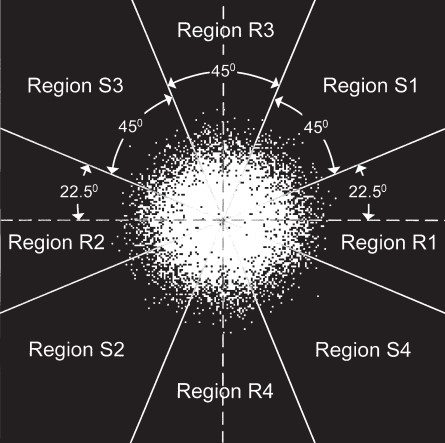
\includegraphics[width=0.45\textwidth]{Figures/Correction algorithm FFT segmentation.jpg}
    \caption{FFT segmentation \cite{SEM correction algorithm}.}
    \label{Correction algorithm FFT segmentation}
\end{figure}

\paragraph{}
The focus can be adjusted by comparing the sum of pixel values in $T$, $T_{uf}$ and $T_{of}$. Let the perfect focus for the image be $\hat{F}$, then
\begin{align*}
\begin{cases}
    \text{sum}(T_{of}) < \text{sum}(T_{uf}), & \hat{F} < F_{uf} < F\\
    \text{sum}(T_{of}) < \text{sum}(T_{uf}), & F_{uf} < \hat{F} < F \\
    \text{sum}(T_{of}) = \text{sum}(T_{uf}), & F = \hat{F} \\
    \text{sum}(T_{uf}) < \text{sum}(T_{of}), & F_{of} > \hat{F} > F \\
    \text{sum}(T_{uf}) < \text{sum}(T_{of}), & \hat{F} > F_{of} > F
\end{cases}.
\end{align*}
Let
\begin{equation}
    P = \text{sum}(T_{of}) - \text{sum}(T_{uf}).
\end{equation}
Then, the rules for adjusting focus are
\begin{itemize}
    \item when $P>0$, the focus should be decreased.
    \item when $P<0$, the focus should be increased.
\end{itemize}

\paragraph{}
After the focus has been set to the perfect value, i.e. when $F=\hat{F}$, the stigmator settings can be adjusted by comparing the sum of pixel values in different regions of $T$, $T_{uf}$ and $T_{of}$. Let
\begin{align}
    P_{R12} & = \text{sum}(T_{of,R12}) - \text{sum}(T_{uf,R12}), \\
    P_{R34} & = \text{sum}(T_{of,R34}) - \text{sum}(T_{uf,R34}), \\
    P_{S12} & = \text{sum}(T_{of,S12}) - \text{sum}(T_{uf,S12}), \\
    P_{S34} & = \text{sum}(T_{of,S34}) - \text{sum}(T_{uf,S34}).
\end{align}
The rules for adjusting the stigmators can be determined from Fig. \ref{SEM astigmatism}. As can be seen in the figure, stigmator x affects the astigmatism in the horizontal and vertical directions, i.e. $P_{R12}$ and $P_{R34}$, and stigmator y affects that in the diagonal directions, i.e. $P_{S12}$ and ${P_{S34}}$. Then:
\begin{itemize}
    \item when $P_{R12}>0$ and $P_{R34}<0$, the value of stigmator x should be decreased.
    \item when $P_{R12}<0$ and $P_{R34}>0$, the value of stigmator x should be increased.
    \item when $P_{S12}>0$ and $P_{S34}<0$, the value of stigmator y should be increased.
    \item when $P_{S12}<0$ and $P_{S34}>0$, the value of stigmator y should be decreased.
\end{itemize}

\section{Practical considerations}
\paragraph{}
The performance of the algorithm is affected by five key parameters:
\begin{itemize}
    \item $P_{threshold}$. Ideally, the focus of the SEM should be set to a value such that $P = 0$, i.e. the under-focused image and the over-focused image have the same FFT magnitude. However, this is practically impossible due to noise, non-linearity in the lens system, etc. Therefore, $P_{threshold}$ is used to define a threshold such that the image is considered to be in perfect focus when $|P| < P_{threshold}$. If $P$ is normalised, $P_{threshold}$ can be conveniently set to a percentage value.
    \item $F_{step}$, which is how much the focus should be adjusted during each iteration in focus adjustment. A smaller $F_{step}$ allows the final image to have a finer resolution but increases the amount of time needed for the adjustment. A larger $F_{step}$ speeds up the process but may never achieve the level of focus as required by $P_{threshold}$. To achieve the best result, larger values of $F_{step}$ should be used at the beginning and smaller ones towards the end.
    \item $\Delta F$, which determines how much the focus should be changed to obtain the under-focused and over-focused images. It is more important to the astigmatism correction step. When $\Delta F$ is too small, the difference between the FFT of the under-focused and over-focused image will not be significant enough and can be easily hidden by noise. When it is too big, the FFTs will lose their high-frequency components, which again makes the difference too small.
    \item $S_{threshold}$. The values of $P_{R12}$, $P_{R34}$, $P_{S12}$, $P_{S34}$ are prone to the influence of noise near zero. Same as the purpose of $P_{threshold}$, $S_{threshold}$ defines a threshold to circumvent this problem.
    \item $S_{step}$, which is how much the value of the stigmator control should be adjusted during each iteration in astigmatism adjustment. Similar to $F_{step}$, it determines the speed of the adjustment and the level of fineness of the final images.
\end{itemize}

\paragraph{}
Another factor that affects the speed of the algorithm is how fast the FFT segmentation can be done. The most straightforward way of doing it is to iterate through the whole matrix while calculating the sums in pure Python, for every FFT. This is slow, and the \textit{Masker} class provides a faster solution.

\paragraph{}
A \textit{Masker} is initialised with a 2D shape, and it creates eight matrices, each representing a region as shown in Fig. \ref{Correction algorithm FFT segmentation}. For example, if the input is $[5, 7]$, the matrix created for region R1 will be
\begin{align*}
\begin{bmatrix}
1 & 1 & 1 & 1 & 1 & 1 & 1\\
1 & 1 & 1 & 1 & 1 & 1 & 0\\
1 & 1 & 1 & 0 & 0 & 0 & 0\\
1 & 1 & 1 & 1 & 1 & 1 & 0\\
1 & 1 & 1 & 1 & 1 & 1 & 1
\end{bmatrix}.
\end{align*}
The code ensures that there is no overlapping between matrices apart from at the center. The sum of values in region R1 of the FFT can be calculated using:
\begin{lstlisting}
ma.array(fft, masker.r1).sum()
\end{lstlisting}

\section{Experiment, results, and discussions}
\paragraph{}
Due to the impact of the COVID-19 pandemic, the algorithm has not been comprehensively tested and only some preliminary experiments were conducted to verify the logic of the algorithm and the correctness of the implementation. Fig. \ref{Correction algorithm test} shows the result of the focusing correction done by the algorithm. It was able to find the same best focus for the SEM as determined by the operator.

\begin{figure}[htbp]
    \centering
    \begin{subfigure}{0.45\textwidth}
        \centering
        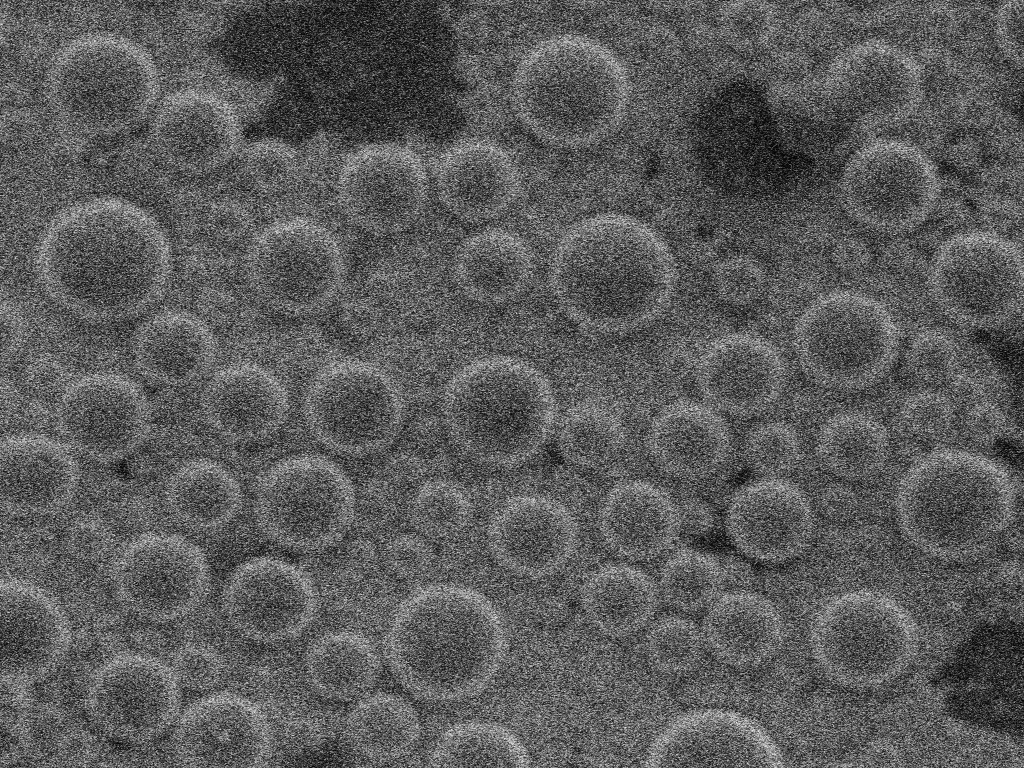
\includegraphics[width=1\textwidth]{Figures/Correction algorithm test initial image.png}
        \caption{Initial.}
    \end{subfigure}
    \begin{subfigure}{0.45\textwidth}
        \centering
        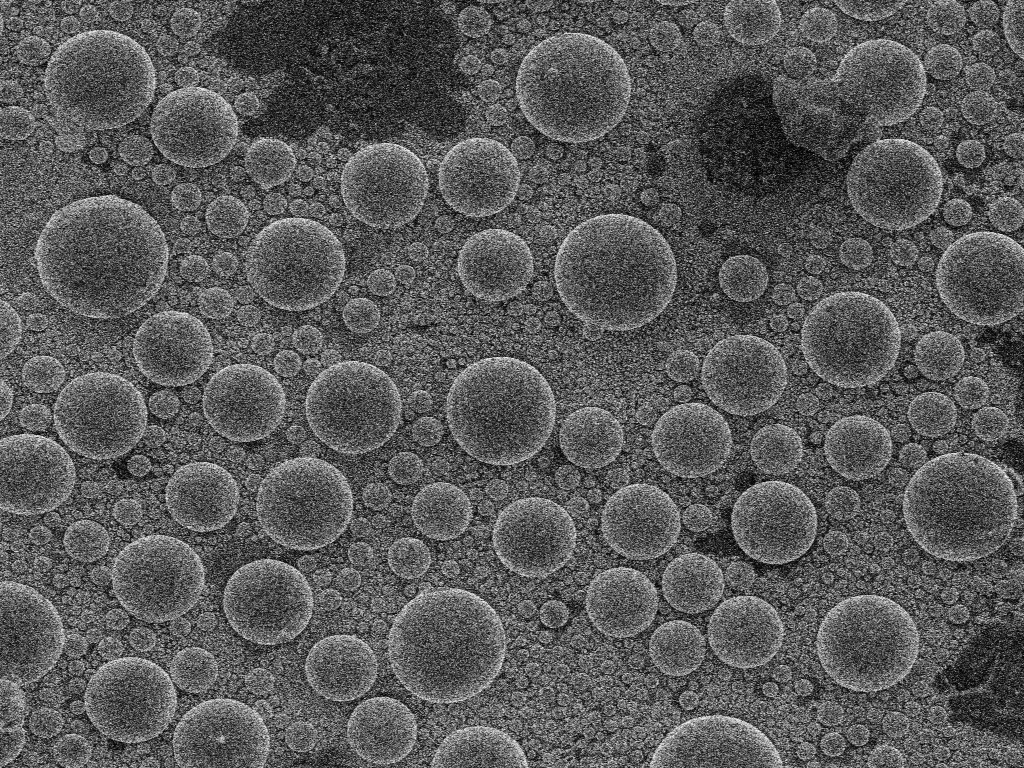
\includegraphics[width=1\textwidth]{Figures/Correction algorithm test final image.png}
        \caption{Final.}
    \end{subfigure}
    \caption{Automatic focusing correction.}
    \label{Correction algorithm test}
\end{figure}

\paragraph{}
A major practical problem found during the experiment is that although the FFTs can be calculated within a few milliseconds using the real-time diagnostic tool, the algorithm still has to wait a few hundred milliseconds in each iteration for the SEM image to be updated. This is because the SEM needs to perform multiple scans on the object and take the average to reduce noise.

\paragraph{}
Another problem is that it is difficult to determine the best values for the five parameters mentioned earlier. The result shown in Fig. \ref{Correction algorithm test} was obtained using the best settings found empirically, which may be dependent on the model of the SEM and characteristics of the object under observation.

\chapter{Conclusions}
\paragraph{}
The GPU can perform some general-purpose computing tasks much faster than the CPU because of its architecture that emphasises on parallelism. Experiments have shown that a common middle-range GPU can perform vector operations about eight times faster than a similarly priced CPU. This has allowed the development of a real-time diagnostic tool for SEMs.

\paragraph{}
The real-time diagnostic tool provides SEM operators a novel way for evaluating the focusing and astigmatism of SEM images, and making corresponding adjustments to the SEM. In the past, operators make judgements based on the stretching of the images. By performing the calculations ten times faster, the use of GPGPU gives operators access to the FFT of the images in real-time at about ten frames per second. This allows operators to evaluate the focusing and astigmatism of SEM images using the FFT, eliminating the subjectivity and difficulty caused by complex structures of the object in the old method.

\paragraph{}
Being real-time also means that the diagnostic tool can be used to support fast automatic algorithms. An algorithm has been implemented and preliminary tests have shown that it is able to correct the focusing of the SEM as good as an SEM operator. Further experiments need to be conducted to verify its ability to correct astigmatism and to further improve its speed.

\begin{thebibliography}{00}
    % \bibitem{SEM for semiconductors}
    % C. REEVES, ``The uses of scanning electron microscopy for studying semiconductor devices,'' International Journal of Electronics, vol. 77, no. 6, pp. 919-928, 1994, doi: 10.1080/00207219408926111.

    % \bibitem{SEM for baterial cells}
    % T. Cushnie, N. O’Driscoll and A. Lamb, ``Morphological and ultrastructural changes in bacterial cells as an indicator of antibacterial mechanism of action,'' Cellular and Molecular Life Sciences, vol. 73, no. 23, pp. 4471-4492, 2016, doi: 10.1007/s00018-016-2302-2.

    \bibitem{SEM for semiconductor inspection}
    ``Review SEM - What is a Review SEM?,'' Hitachi, [Online], available: \url{https://www.hitachi-hightech.com/global/products/device/semiconductor/review-sem.html}. [Accessed: 25 May 2020]

    % \bibitem{SEM applications}
    % ``The Applications and Practical Uses of Scannning Electron Microscopes,'' ATA Scientific Instruments, 2019, [Online], available: \url{https://www.atascientific.com.au/sem-imaging-applications-practical-uses-scanning-electron-microscopes/}. [Accessed: 25 May 2020]

    \bibitem{SEM A to Z}
    ``SEM A to Z,'' Jeol.co.jp, [Online], available: \url{https://www.jeol.co.jp/en/applications/pdf/sm/sem_atoz_all.pdf}. [Accessed: 18 May 2020].

    \bibitem{SEM image sharpness measurement}
    A. Vladár, M. Postek and M. Davidson, ``Image sharpness measurement in scanning electron microscopy-part II,'' Scanning, vol. 20, no. 1, pp. 24-34, 2006, doi: 10.1002/sca.1998.4950200104.

    \bibitem{GPU computing}
    J. D. Owens, M. Houston, D. Luebke, S. Green, J. E. Stone and J. C. Phillips, ``GPU Computing,'' in Proceedings of the IEEE, vol. 96, no. 5, pp. 879-899, May 2008, doi: 10.1109/JPROC.2008.917757.

    \bibitem{Deep learning}
    Ian Goodfellow; Yoshua Bengio; Aaron Courville, ``Deep learning,'' in Deep Learning, The MIT Press, 2017, p. 23.

    \bibitem{GPU architecture lecture}
    ``GPU Architecture and CUDA Programming,'' Carnegie Mellon University, 2017, [Online], available: \url{http://15418.courses.cs.cmu.edu/spring2017/home}. [Accessed: 19 May 2020].

    \bibitem{FT FFT}
    J. Cooley and J. Tukey, ``An algorithm for the machine calculation of complex Fourier series,'' Mathematics of Computation, vol. 19, no. 90, pp. 297-297, 1965, doi: 10.1090/s0025-5718-1965-0178586-1.

    \bibitem{FT lecture}
    ``2D Fourier transforms and applications,'' University of Oxford, 2014, [Online], available: \url{http://www.robots.ox.ac.uk/}. [Accessed: 19 May 2020].

    \bibitem{SEM astigmatism correction}
    C. Lyman, ``Correcting Astigmatism in SEM Images,'' Microscopy Today, vol. 27, no. 03, pp. 32-35, 2019, doi: 10.1017/s1551929519000476.

    \bibitem{SEM correction algorithm}
    K.H. Ong, J.C.H. Phang and J.T.L. Thong, ``A robust focusing and astigmatism correction method for the scanning electron microscope,'', scanning 19: 553-563, 1997, doi: 10.1002/sca.4950190805.
\end{thebibliography}
\end{document}
